%
% File: introduction.tex
% Author: Eshwen Bhal
% Description: Introductory chapter.
%
\let\textcircled=\pgftextcircled
\chapter{Introduction}
\label{chap:intro}

% Hard to describe dark matter as an object. Do I call it a 'substance', 'thing', 'mass'? Can refer to it as 'non-luminous' if struggling for other adjectives

\initial{T}he universe, in all its vastness, structure, natural laws and chaos, is comprised of only three principal components: visible matter, the ingredients of stars, planets and life, is the only one we interact with on a regular basis; dark energy, a force or manifestation of something even more mysterious, responsible for the accelerating expansion of the universe, is almost entirely unknown; and dark matter, a substance invisible in all sense of the word, that binds galaxies together and influences large scale structure in the cosmos, is the focus of this thesis.


%=========================================================


\section{Evidence for dark matter}
\label{sec:intro_dm_evidence}

The earliest evidence for a large, non-luminous component of the galaxy stretches back to the 1920s when Jacobus Kapteyn attempted to explain the motion of stars in the Milky Way~\cite{1922ApJ....55..302K}. Since then, a wealth of independent astrophysical observations have reinforced the existence of this aggregation not just in our own, but in countless other galaxies and cosmological bodies. The Coma Cluster is a famous example: 90\,\% of its mass is thought to arise from dark matter, confirmed by its large mass-to-light ratio of 400 $M_{\odot} / L_{\odot}$~\cite{Yozin:2015mla}. Further evidence is that the rotation curves of most galaxies are roughly flat \cite{1996MNRAS-281-27P}, contrary to the expected Keplerian curve ($v \propto 1/\sqrt{r}$) expected from solely visible matter. On a galactic scale, dark matter is sprinkled in a mostly spherical halo that spans beyond the observable disc. The inclusive dark matter mass increases linearly~\cite{2009arXiv0901.0632E} to compensate for the decline expressed by visible matter~\cite{1970ApJ-160-811F,1992AandA-256-19B}. Gravitational lensing is another observational tool subject to be influenced by dark matter. Images of galaxies and other objects captured by this method appear distorted from a large gravitational field between the source and observer warping its local spacetime~\cite{2010GReGr..42.2177H}. Arcs, ellipses and Einstein rings of smeared galaxies are often seen when dark matter is present.

While there are no widely-accepted estimations, it is believed that 85$-$95\,\% of the Milky Way is comprised of dark matter~\cite{2005MNRAS.364..433B,2006MNRAS.370.1055B,Kafle:2014xfa}. Though these approximations include non-visible identifiable matter such as dim stars, black holes and neutron stars, the term ``dark matter'' typically reserved for the non-luminous, \emph{non-baryonic} segment that pervades the cosmos. From the latest results of the Planck mission, the energy density of the observable universe is composed of 26.5\,\% dark matter~\cite{Aghanim:2018eyx}. This result follows the Lambda cold dark matter ($\Lambda\text{CDM}$) model to describe the constituents and evolution of the universe, which is often referred to as the cosmological analog of the \acrlong{sm} of particle physics (\acrshort{sm}). From the calculations, postulations, and observations presented above, the following properties of dark matter can be deduced:

\begin{easylist}[itemize]
\ListProperties(Style*=-- , FinalMark={)}) % FinalMark indicates the end of the list properties and must always be used
& It is electrically neutral since it does not interact with electromagnetic radiation.
& It is cold (non-relativistic). Its velocity within galaxies is similar to the inhabiting stars~\cite{Herzog-Arbeitman:2017fte,Bhattacharjee:2012xm}, since the combination of visible and dark matter drives the measured rotation curves. One small caveat is that galactic dark matter would be cold since a velocity above the gravitational escape velocity of the galaxy would eject high speed particles.
& It is stable, at least on the timescale of the current age of the universe. Dark matter production is postulated to have occurred only in the early universe via a thermal freeze out mechanism (see Chpt.~\ref{sec:theory_dark_matter}). Hence, the remaining fraction has been present for a considerable time. Since most galaxies are dominated by dark matter and the gravitational influence from only the visible matter is too small to maintain itself, they could not have developed with out it. This supports the idea of ``bottom-up'' structure formation in the universe; smaller galaxies form around gravitational potential wells provided by coalescing dark matter, then merge to form larger structures~\cite{doi:10.1093-mnras-183.3.341}.
& Its interaction with matter and itself is very weak, or even non-existent. The Bullet Cluster --- an astronomical object encompassed by two colliding galaxy clusters --- is the best example of this inference. From measurements of predominantly x-ray emission and gravitational lensing, it was found that while there is substantial dark matter present, interaction with itself and the visible matter surrounding it was minimal at most~\cite{BulletClusterDMevidence}. A kinematic explanation for the spherical distribution and low velocity of dark matter in galaxies can be explained by its collisionless nature. During the formation of a galaxy or stellar system, visible matter frequently collides, dissipating angular momentum and collapsing into a disc.
\end{easylist}


%=========================================================


\subsection{Alternative theories to dark matter}
\label{subsec:intro_alternative_dm_theories}

Though little is known about dark matter itself since all evidence stems from its gravitational influence, there are alternative theories that may explain the observations presented above. However, the scientific community can exclude many of these. Mismeasurements of the amount of baryonic matter such as neutrinos, neutrons, and interstellar gas are among the simpler propositions.

The neutrino flux from stars, as well as the cosmic neutrino background~\cite{weinberg2008cosmology}, are precise and well-tested [REF]. Even considering the upper limits on neutrino masses~\cite{1742-6596-718-2-022013}, they cannot make a significant contribution to the dark matter content in the universe. This is even discounting their highly relativistic nature, where myriad experimental evidence suggests dark matter is cold.

One can also use the Cosmic Microwave Background to calculate the average photon and neutrino densities, and Big Bang Nucleosynthesis calculations to determine the baryonic matter density (see Ref.~\citenum{Fields:2019pfx} for results with the latest Planck mission data). These can be compared to other measurements, e.g., mass-to-light ratios averaged across the universe, to reveal a discrepancy~\cite{cox2016universal}.

Neutrons cannot contribute to dark matter because isolated neutrons are unstable, decaying in a matter of minutes~\cite{PDGbooklet2010}. Transforming into charged protons and electrons, they interact strongly with light and therefore contribute to the luminous matter content.

\Gls{mond} is a hypothesis that aims to explain phenomena typically associated with dark matter instead by modifications to Newton's laws of motion. There exist many theories and interpretations derived from this principle, though any one strand that tries to explain an observation usually fails to satisfy other phenomena or apply to length scales that general relativity may predict well. For example, observations of the Bullet Cluster~\cite{BulletClusterDMevidence} have discredited many popular \acrshort{mond} models.


%=========================================================


\section{Overview of dark matter searches}
\label{sec:intro_dm_searches}

While observational evidence has so far lain with astrophysics, a theoretical description and discovery of dark matter may fall into the realm of particle physics with the numerous, novel experimental searches underway.  The detection of dark matter can be classified into three distinct methods with unique signatures (with a visual summary in Fig. \ref{fig:dm_detection_methods}):

\begin{easylist}[itemize]
\ListProperties(Style*=-- , FinalMark={)})
& \textbf{Direct}: dark matter may interact with visible matter on small scales, scattering \acrshort{sm} particles~\cite{Schumann:2019eaa}. The recoil these \acrshort{sm} particles experience could be detected by highly-sensitive, low background experiments such as \acrfull{lz}~\cite{Akerib:2019fml} that specialises in the search for \acrshort{wimp} dark matter at a large range of masses.
& \textbf{Indirect}: if dark matter interacts with itself, it may annihilate to produce showers of high energy photons or pions. Background estimation is difficult since the signatures can be highly model-dependent. The photons may be of a continuum --- from hadronisation and radiation of the decay products --- or contain features, such as internal radiation from the propagator in the interaction or from loop-level processes~\cite{Conrad:2017pms}. Large ranges of the annihilation cross section and dark matter mass can be probed with telescopes already searching for these characteristic events.
& \textbf{Production}: dark matter may have been abundantly produced in the hot, early universe. High energy particle accelerators such as the \acrshort{lhc} can reproduce these conditions, with the \acrshort{wimp} miracle (see Chpt.~\ref{sec:theory_dark_matter}) reinforcing the idea that dark matter may exist in these accessible mass ranges. Many \acrfull{bsm} theories accommodate dark matter candidates with a diverse spectrum of final states that can be investigated by analysing \acrshort{lhc} data.
\end{easylist}

\begin{figure}[htbp]
    \centering
    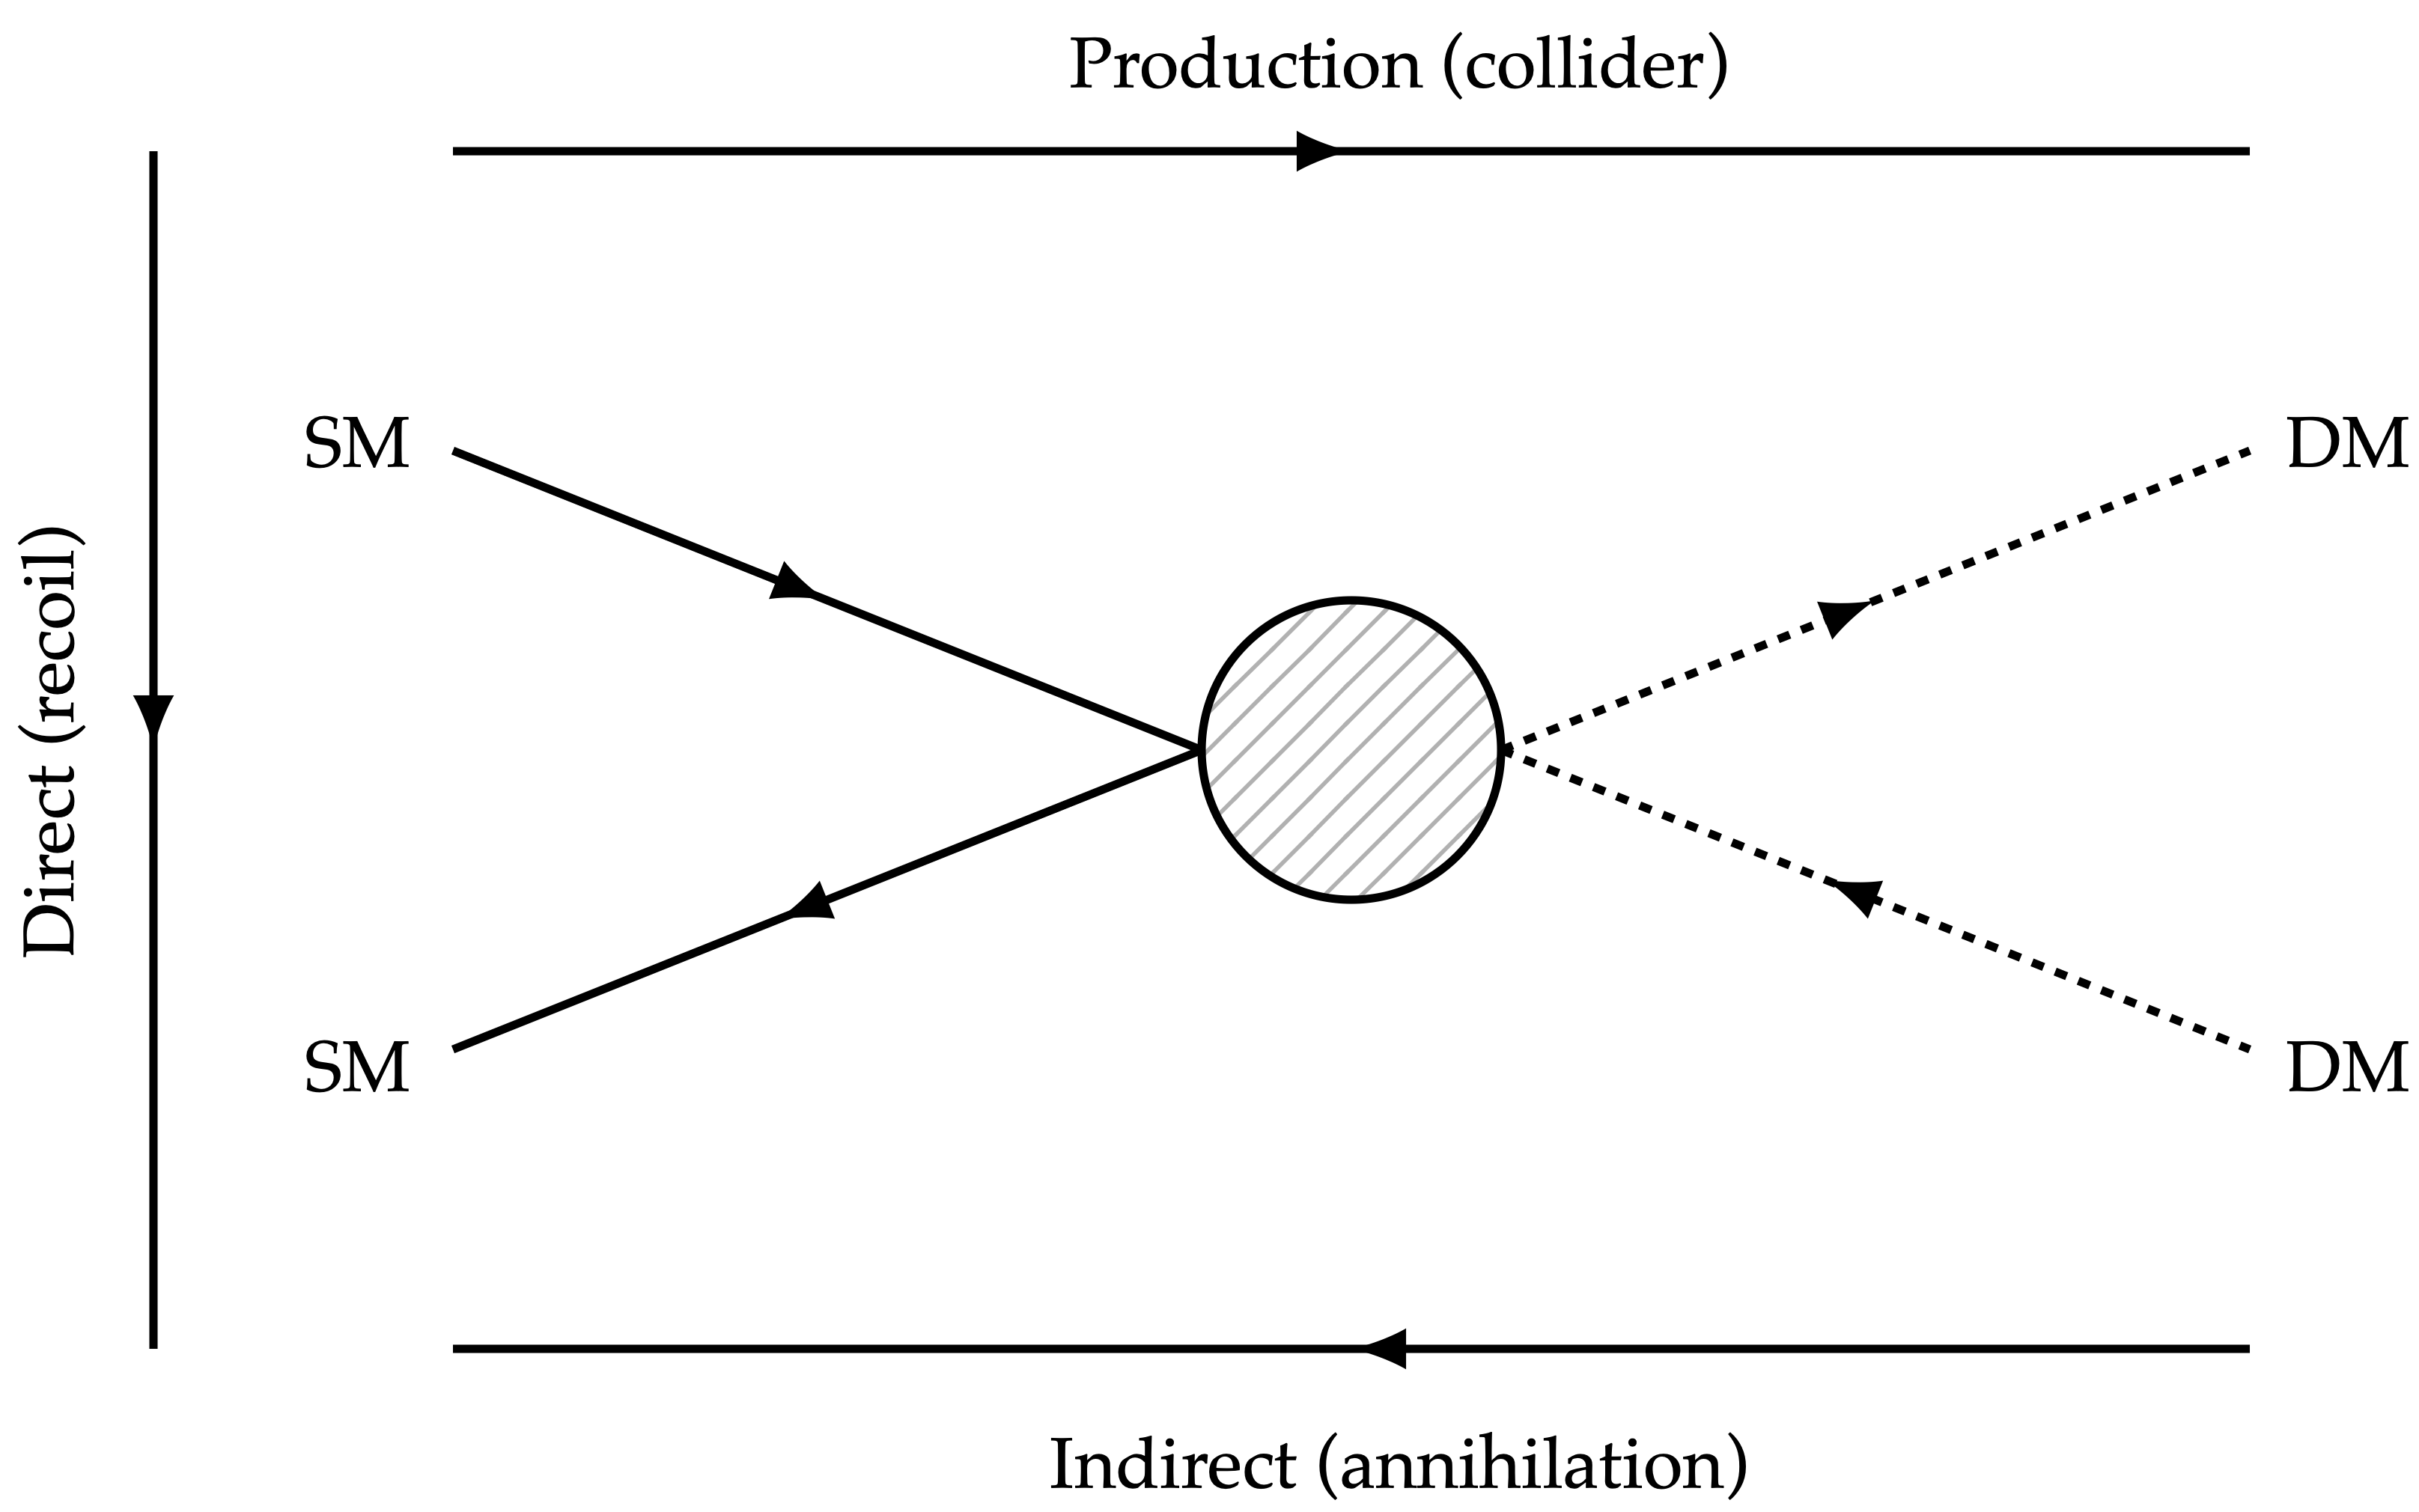
\includegraphics[width=0.75\textwidth]{figures/DM_detection_methods.png}
    \caption[A visual representation of the three main types of dark matter detection: direct, indirect, and production]{A visual representation of the three main types of dark matter detection: direct (dark matter recoiling from \acrlong{sm} particles); indirect (annihilation of dark matter); and production (dark matter created in high energy physics collisions).}
    \label{fig:dm_detection_methods}
\end{figure}


%=========================================================


\subsection{Dark matter searches at the LHC}
\label{subsec:dm_searches_lhc}

Since its detection at the \acrshort{cms} experiment from the production mechanism is the focus of this thesis, it is important to establish the current state of dark matter searches at the \acrfull{lhc}, the world's most powerful particle accelerator that provides data for \acrshort{cms}. Both machines are described in detail in Chpt.~\ref{chap:detector}, and as such only a summary will be provided here. The \acrshort{lhc} principally collides protons at centre of mass energies up to \comruntwo. These exceptionally high energies allow the conditions in the very early universe to be simulated in which heavy, unstable particles were created in abundance. As such, many theories can be investigated that postulate heavy particles that do not exist in the universe today. Some of these, such as \acrfull{susy} \cite{Martin:1997ns}, sterile neutrinos \cite{doi:10.1142/S0218301313300191}, and Kaluza-Klein states \cite{Han:1998sg} contain dark matter candidates that can be specifically searched for, or indirectly discovered if a theory is experimentally proven. Despite the success of the \acrlong{sm} in explaining the natural world, it does not substantiate the existence of dark matter; hence why \acrshort{bsm} theories are popular. Fig.~\ref{fig:dm_masses_xsecs} illustrates the masses and interaction cross sections of many dark matter candidates. \Glspl{wimp} (highlighted by the purple rectangle) are the the subject of many searches at the LHC since the expected mass ranges and cross sections are accessible there.

\begin{figure}[htbp]
    \centering
    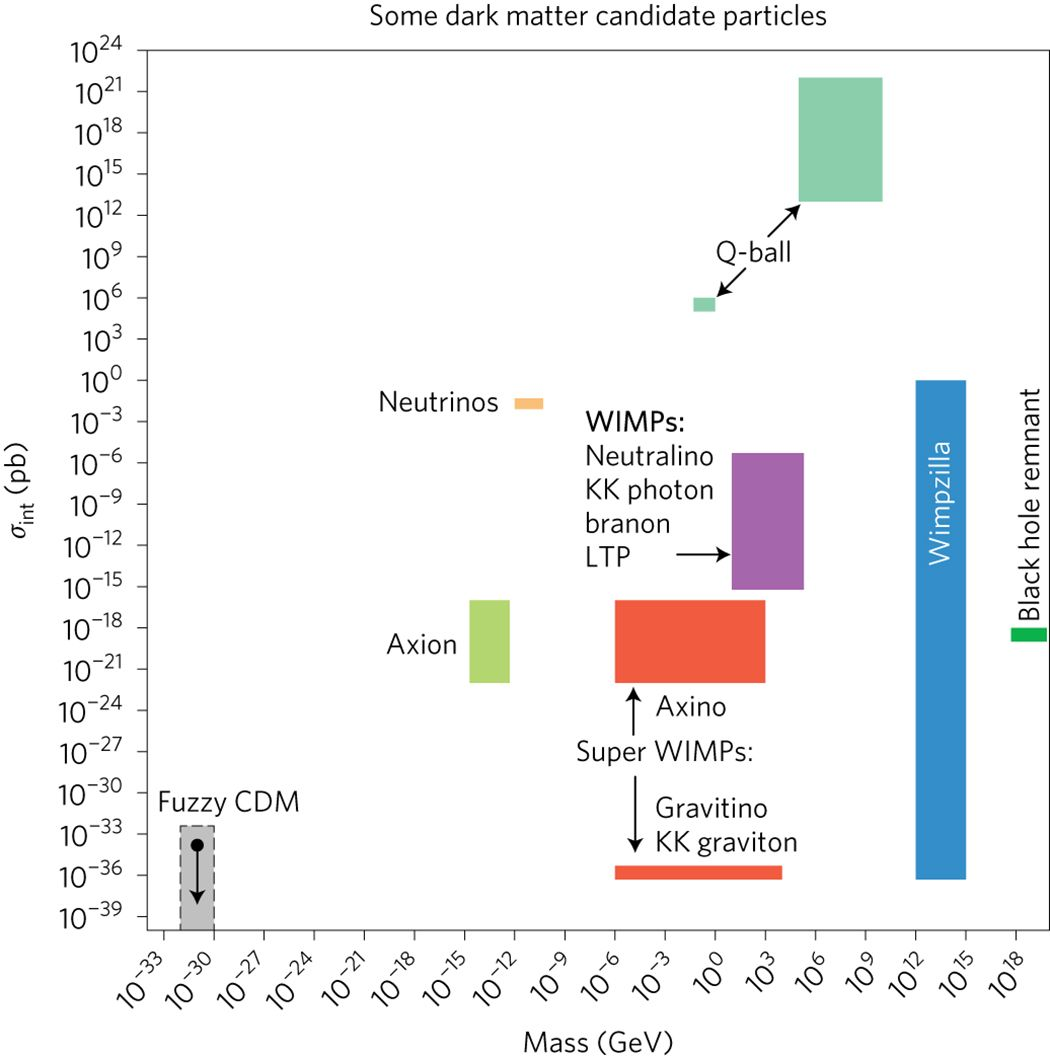
\includegraphics[width=0.6\textwidth]{figures/dm_masses_xsecs.jpg}
    \caption[The expected masses and interaction cross sections of some dark matter candidates. The centre of mass energy of the LHC is best suited to targeting \glspl{wimp}]{The expected masses and interaction cross sections of some dark matter candidates. The centre of mass energy of the LHC is best suited to targeting \glspl{wimp}. Figure acquired from Ref.~\citenum{Conrad:2017pms}.}
    \label{fig:dm_masses_xsecs}
\end{figure}

Two avenues are usually considered when attempting to discover dark matter: explicit searches for the signatures of dark matter production, and anomalies in precision measurements. The former is quite common, with many theories and models tested at the LHC's general purpose detectors, \acrshort{atlas} and \acrshort{cms}. Searches at CMS have been performed for promptly-decaying and ``long-lived'' \acrlong{susy} in hadronic final states (in which I made contributions) \cite{CMS-PAPER-SUS-15-005-published,SUS16038published}. Searches for specific supersymmetric particles in a variety of decay modes have been conducted by both experiments \cite{CANEPA2019100033}. In many of these cases, the \acrfull{lsp} is considered to be a dark matter candidate. $R$-parity conservation is predicted (or even enforced) in many \acrshort{susy} models \cite{Martin:1997ns}, which prevents the decay of \acrshort{lsp} and any lighter, \acrlong{sm} particles that have been observed to be stable. While \acrlong{susy} is the most popular \acrshort{bsm} theory, due in part to its numerous interpretations and approaches for discovery, many others have also been explored at the LHC. From microscopic black holes \cite{Khachatryan:2010wx}, to [OTHERS], there are many strategies that have the potential to uproot the \acrlong{sm}. The analyses above are usually characterised by large ``missing'' transverse momentum (explained further in Chpt. \ref{subsec:theory_met}), a quantity that represents the momenta of particles invisible to the detector, which include dark matter. In Chpt. \ref{chap:svj}, I discuss in detail a search for dark matter that utilises this variable.

Precision measurements of \acrlong{sm} parameters is the other method often consulted in the hopes of attributing anomalies to new physics. For example, attempts to explain anomalies in the $\Pqb \rightarrow \Pqs$ transition include dark matter candidates \cite{anomalies_b_s_dark_matter,another_b_s_anomaly_paper}. In Chpt. \ref{chap:higgstoinv}, I investigate how the measurement of the Higgs boson to invisible state branching ratio can accommodate dark matter. \footnote{Maybe add another example of anomalies in precision measurements}

There is significant motivation to study dark matter from a wider, as well as a more personal, viewpoint. It is important to understand how the universe operates, and dark matter opens up the potential for new physics that improves our understanding of nature. My personal interests include the blend of particle physics and astrophysics, and the opportunity to discover and add to humanity's collective wisdom. With 137\,\fbinv from CMS during Run-2 at \comruntwo, there is great potential to constrain some of the properties of dark matter. This thesis showcases the motivation for, and results of, searches for invisibly decaying Higgs bosons and \glspl{svj} with the full Run-2 dataset collected by the CMS experiment. \footnote{Add another figure or two somewhere to help separate the text? Maybe an astronomical image of the Bullet Cluster/dark matter distribution in a cosmological object, or a gravitational lensing ring from dark matter}

%=========================================================
